\documentclass[preprint, 10pt]{elsarticle}

\newcommand{\mcaption}[2]{\caption{\small \em #1}\label{#2}}
\newcommand{\secref}[1]{\ref{#1}}

\usepackage{amsfonts}
\usepackage[fleqn,reqno]{amsmath}
\usepackage{amssymb}
\usepackage[titletoc]{appendix}
\usepackage{enumitem}
\usepackage{filecontents}
\usepackage[top=1.2in,bottom=1.2in,left=1in, right=1in]{geometry}
\usepackage{graphics}
\usepackage{lineno}
%\usepackage{showkeys} %To see the labels for now.  Will remove later
\usepackage{pgfplots}
\usepackage{tikz}
\usepackage{todonotes}

\usetikzlibrary{arrows}


%%%%%%  pdftex  %%%%%%%%%%%%%%%%%%%%%%%%%%%%%%%%%%%%%%%%%%%%%%%%%%%%%%
\usepackage[pagebackref=false,bookmarks=false]{hyperref} 

\hypersetup{
  bookmarksnumbered=true,
  bookmarksopen=false,
  hypertexnames=false,      
  breaklinks=true,          
  unicode=false,
  pdffitwindow=true,        
  pdfnewwindow=true,        
  colorlinks=true,         
  linkcolor=dblue,
  anchorcolor=red,
  citecolor=dorange,
  filecolor=magenta,
  urlcolor=dblue,
  pdfstartview = FitH,
  pdfkeywords = {},
  pdfcreator = {LaTeX with hyperref package}
}

\newcommand{\bd}{{\partial}}
\newcommand{\cc}{{\mathbf{c}}}
\newcommand{\DD}{{\mathcal{D}}}
\newcommand{\eeta}{{\boldsymbol\eta}}
\newcommand{\ff}{{\mathbf{f}}}
\newcommand{\grad}{{\nabla}}
\newcommand{\llambda}{{\boldsymbol\lambda}}
\newcommand{\nn}{{\mathbf{n}}}
\newcommand{\NN}{{\mathcal{N}}}
\newcommand{\pderiv}[2]{\frac{\partial #1}{\partial #2}}
\newcommand{\rr}{{\mathbf{r}}}
\newcommand{\RR}{{\mathbb{R}}}
\renewcommand{\ss}{{\mathbf{s}}}
\newcommand{\ssigma}{{\boldsymbol\sigma}}
\newcommand{\uu}{{\mathbf{u}}}
\newcommand{\UU}{{\mathbf{U}}}
\newcommand{\vv}{{\mathbf{v}}}
\newcommand{\xx}{{\mathbf{x}}}
\newcommand{\xxi}{{\boldsymbol{\xi}}}
\newcommand{\yy}{{\mathbf{y}}}


\begin{document}

\title{A stable, contact-free, time stepping method for rigid particle suspensions}

\author[Lukas]{Lukas Bystricky}
\author[Lukas]{Sachin Shanbhag}
\author[Bryan]{Bryan D.~Quaife}
\address[Lukas]{Department of Scientific Computing, Florida State University,
Tallahassee, FL, 32306.}
\address[Bryan]{Department of Scientific Computing and Geophysical Fluid
Dynamics Institute, Florida State University, Tallahassee, FL, 32306.}

\begin{abstract} 
We consider suspensions of rigid bodies in two dimensions in a viscous fluid. The governing Stokes equations prohibit contact between particles in finite time, however in practice, insufficient spatial and temporal discretization can lead to contact and overlap between particles. Repulsion forces can be used to used to avoid such collisions. By quantifying the amount of overlap between particles, the direction and magnitude of these forces can be determined in such a way as to explicitly guarantee that no collisions are possible. This paper builds on a recent work by Lu \emph{et al}. In their paper interactions between different particles are treated explicitly. This can lead to stiffness, in particular for dense suspensions. Instead, we treat the interactions between all particles implicitly, thereby reducing the stiffness of the time stepper and allowing us to model more concentrated suspensions while maintaining a reasonably large time step size. We demonstrate this method on various unbounded and bounded flows and use it to compute rheological properties. 

\end{abstract}

\begin{keyword}
  Stokes flow \sep Boundary integral method \sep Rigid body suspensions 
\end{keyword}

\maketitle


%%%%%%%%%%%%%%%%%%%%%%%%%%%%%%%%%%%%%%%%%%%%%%%%%%%%%%%%%%%%%%%%%%%%%%%
\section{Introduction\label{s:intro}}
Dispersions of particulate rods or fibers are used in composite
materials to tune mechanical, thermal, and electrical properties.
Typically, these materials are processed in the melt or liquid
suspension state via operations like injection molding, extrusion,
casting, etc. It is important to model fiber suspensions for two
reasons: (i) the distribution and orientation of the fibers, which
determines the properties of the composite material, are governed by the
flow history during processing, and (ii) the rheological properties of
the suspension, which influence the flow behavior, in turn, depend on
the size, shape, distribution, and orientation of the
fibers~\cite{larsoncf}.

The theory of rigid fibers in flowing fluids was pioneered by
Jeffery~\cite{Jeffery1922} who analyzed the motion of a single
spheroidal particle sheared in a Newtonian solvent. At a given shear
rate $\dot{\gamma}$, he observed that fibers of length $\ell$ and diameter
$d$, underwent periodic motion with a period $(\pi/\dot{\gamma})
(\lambda + 1/\lambda)$, where $\lambda = \ell/d$ is the aspect ratio. The
period increases with $\lambda$, and when $\lambda \gg 1$ a particle
exhibiting ``Jeffery's orbit" stays aligned with the flow direction most
of the time, before abruptly spinning through a half-revolution. In the
dilute regime (number of rods/unit volume $\nu < 1/\ell^3$), trajectories
of elongated fibers of different shapes, such as cylinders, can be
quantitatively described via Jeffery's orbits once corrections are made
for particle shape~\cite{Bretherton1962}.

As $\nu$ increases, the interactions between fibers become significant.
Batchelor extended Jeffery's theory for multiple particles, by relating
the average stress tensor, ${\bm \sigma}$, to the distribution of fiber
orientation $\mathbf{p}$, and the deformation tensor $\mathbf{D} =
(\nabla \mathbf{u} + \nabla \mathbf{u}^\intercal)/2$. Assuming purely
hydrodynamic interactions between fibers, and a slender body
approximation ($\lambda \gg 1$)~\cite{Batchelor1970, Batchelor1970a,
Doi1978, Dinh1984, Shaqfeh1990},
\begin{align}
  {\bm \sigma} = 2 \mu \mathbf{D} + \nu \zeta 
    \langle \mathbf{p p p p} \rangle : \mathbf{D},
\label{eqn:batchelor}
\end{align}
where $\mu$ is the solvent viscosity, and $\zeta$ is a drag
coefficient~\cite{Batchelor1971} that depends on the size and
concentration of the particles, and the solvent viscosity. The ensemble
average $\langle \cdot \rangle = \int \cdot \,
\psi(\mathbf{p})\,d\mathbf{p}$ represents a weighted average over the
probability distribution of particle orientations $\psi(\mathbf{p})$. 

In computer simulations, the fiber orientation distribution is modeled
implicitly or explicitly. In the \emph{implicit} approach, individual
fibers are not explicitly represented; instead it relies on averages of
second- and fourth-order fiber orientation tensors, $\langle \mathbf{p
p} \rangle$ and $\langle \mathbf{p p p p} \rangle$. Fluid flow equations
(Stokes or Navier-Stokes) are coupled with evolution equations for the
fiber orientation tensors. In order to solve the resulting equations,
fiber interaction models and closure approximations have to be specified
externally~\cite{Advani1987, Advani1990, Ferec2014, Perez2017}. This is
in contrast to direct numerical simulations where individual fibers are
\emph{explicitly} represented. Typically, fibers are modeled as
prolate ellipsoids~\cite{Ausias2006}, a set of connected
beads~\cite{Yamamoto1996, Joung2001} or rods~\cite{Schmid2000,
Lindstroem2007}, or a slender body ($\ell \gg d$)~\cite{Fan1998,
Rahnama1995, tor-she2004, tor-gus2006, gus-tor2009}, with suitable
first-order corrections to account for finite width. Over the years, in
addition to long-range hydrodynamic interaction, these models have been
supplemented with detailed physics including short-range lubrication,
mechanical contact, and frictional forces~\cite{Sundararajakumar1997,
Lindstroem2008}.

In the semi-dilute regime, $1/\ell^3 \ll \nu \ll 1/d\ell^2$, fiber rotation is
hindered; however, it is found that the static properties are not
significantly altered from the dilute regime~\cite{larsoncf}.
Hydrodynamic interactions between particles dominate the response, and
contacts between fibers are rare. Batchelor's theory, suitably modified
for multibody hydrodynamic interactions~\cite{Shaqfeh1990,
Mackaplow1996}, describes the empirically observed increase in shear
viscosity as a function of $\nu$ reasonably well~\cite{Stover1992,
Bibbo1987, Petrich2000}. The contribution of the fibers to the steady
shear viscosity is relatively modest in non-Brownian suspensions. This
is especially true for high aspect ratio fibers which rotate and align
along the flow direction, and contribute to the viscosity only during
the occasional tumble~\cite{larsoncf}.  Thus, one ought to be careful
not to interpret the success of theory and computer models in predicting
the viscosity change in the semi-dilute regime as validation of the
underlying fiber interaction model. Indeed fiber-fiber interactions are
more sensitively reflected in other viscometric functions such as first
normal stress difference, and distribution of orientations as reflected
in, for example, the dispersion of Jeffery's
orbits~\cite{Lindstroem2009}.

Once the concentration increases beyond $\nu \approx 1/d\ell^2$, the
suspension enters the concentrated regime. Here excluded volume
interactions become important and isotropic packing becomes increasingly
difficult. In this regime, Batchelor's slender body theory and
constitutive relation~\eqref{eqn:batchelor} are no longer valid as
mechanical contacts between fibers start to dominate the response. When
these mechanical interactions are explicitly accounted for, computer
models are able to reproduce a nonzero first normal stress difference
that is observed in experiments~\cite{Sundararajakumar1997, Ausias2006,
Lindstroem2008}. Unlike the dilute and semi-dilute regimes, equation
\eqref{eqn:batchelor} can no longer be used to estimate rheological
properties. Instead, stresses in the suspension have to be computed by
directly summing the forces acting on the fibers~\cite{Ausias2006,
Lindstroem2008}.

In this work, we develop and test tools for two-dimensional direct
numerical simulations of rigid bodies suspended in a viscous fluid.  We
do not make any rigid body assumptions, but rather fully resolve the
fiber shape.  To perform the simulations, we use a boundary integral
equation (BIE) since it resolves the complex geometry by reducing the
set of unknowns to the one-dimensional closed curves that form the fluid
boundary.  Moreover, our BIE fluid solver achieves high-order accuracy.
However, because of numerical errors, without additional techniques,
rigid bodies often unphysically come into contact.  Therefore, we apply
a contact algorithm that allows rigid fibers to come very close to one
another (this happens physically), but guarantees that contact is
avoided without introducing significant stiffness.  In addition to
computing fiber trajectories, we compute rheological and statistical
properties of the fluid and fibers to better understand the dispersion
of fibers in composite materials.

%This is a methods paper
%\begin{itemize}
%  \item Boundary integral equation formulation
%  \item STIV
%  \item FMM
%  \item Near-singular integration
%  \item Pressure and energy dissipation calculations
%  \item Time integrator
%\end{itemize}

\paragraph{Contributions} The main contribution is that we extend the
time stepping strategy introduced for vesicle
suspensions~\cite{Quaife2014} to rigid body suspensions.  Deformable
bodies, such as vesicles, typically maintain a minimum separation
distance, and applying time stepping methods to the velocity due to only
the hydrodynamics results in stable simulations.  However, for rigid
bodies, their proximity can be orders of magnitude smaller than
deformable capsules.  Even with a high-order solver for the fluid
equations and high-order semi-implicit time stepping methods for the
fibers' dynamics, collisions occur because of numerical errors.
Therefore, we use a collision algorithm developed by Lu et
al.~\cite{Lu2017} which guarantees a minimum separation distance between
bodies. In Lu's work, the interaction between different bodies is
treated explicitly.  That is, if $\uu_j$ is the velocity induced by body
$j$, then the time stepping method used is
\begin{align*}
  \frac{\xx_i(t + \Delta t) -  \xx_i(t)}{\Delta t} = \uu_i(t+\Delta t) +
    \sum_{j \neq i} \uu_j(t).
\end{align*}
By treating the interactions between different bodies explicitly, the
minimum separation distance must be kept sufficiently large to avoid
a small time step restriction due to stiffness---a typical minimum
separation distance is $\mathcal{O}(1)$ arclength spacings.  In line
with previous work of one of the authors~\cite{Quaife2014}, we
discretize both inter- and intra-fiber interactions semi-implicitly
\begin{align*}
  \frac{\xx_i(t + \Delta t) -  \xx_i(t)}{\Delta t} = \uu_i(t+\Delta t) +
    \sum_{j \neq i} \uu_j(t+\Delta t).
\end{align*}
With this modification, we are able to take much smaller collision
parameters with introducing excessive stiffness---a typical minimum
separation distance is $\mathcal{O}(10^{-2})$ arclength spacings.

With our new time stepping method, our contact algorithm is applied less
often than the required if interactions are treated explicitly.
Nonetheless, by applying the contact algorithm, the reversibility of the
incompressible Stokes equations is broken.  We systematically examine
the effect of the collision algorithm on the reversibility of the
simulations.

With the ability to do more realistic suspensions of rigid bodies, we
can examine the rheological properties of rigid body suspensions.  In
particular, we effective viscosity of a suspension of rigid bodies in a
Couette device and examine the effect of the suspension's area fraction
and the body's aspect ratio.  Motivated by simulations and analysis by
others~\cite{}, we also examine the statistical properties of the
suspensions.  We are particularly interested in the alignment angle of
fibers.

\paragraph{Limitations} The main limitation is that the method is
developed in two-dimensions.  By limiting ourselves to two-dimensions,
we are able to perform simulations of denser suspensions with high-order
accuracy.  However, many of the algorithms we present have been
developed for rigid bodies three dimensions including boundary integral
equation methods and fast summation methods~\cite{cor-gre-rac-vee2017,
kli-tor2014, kli-tor2016}.  The most challenging algorithms that must be
extended to three dimensions include efficient preconditioners and the
space-time interference volume that requires integrating a
four-dimensional domain ($3$ space dimensions and $1$ time dimension).


\paragraph{Related work} Rather than giving an exhaustive list of work
related to particulate suspensions in viscous fluids, we focus on
literature that is related to BIEs and time stepping to simulate rigid
body suspensions.  A more general overview of BIEs for particulate
suspensions can be found in the texts~\cite{Pozrikidis1992, Guazzelli2011, Karrila1991}.  This work
draws heavily from methods developed for simulating two dimensional
vesicle suspensions~\cite{Quaife2014, Quaife2015, qua-bir2016,
Rahimian2010, Lu2017}.  We represent the velocity as a completed
double-layer potential representation~\cite{Power1987, Power1993,
Karrila1989} that is discretized with a Nystr\"om method using the
trapezoid rule~\cite{Trefethan2014} and solved iteratively with
GMRES~\cite{Saad1986}.  Alternatively, a Galerkin discretization is
possible~\cite{Mammoli1999, Mammoli2002, Mammoli2006}.

Particular algorithmic challenges with BIE formulations, especially for
dense suspensions, are resolving hydrodynamic interactions between
nearly-touching bodies, reducing the cost of the matrix-vector
multiplication required at each GMRES iteration, and reducing the total
number of required iterations.

We avoid weakly-singular integrands by using a double-layer potential,
but nearly-singular integrands are unavoidable in dense suspensions.  We
apply a interpolation-based quadrature method~\cite{Ying2006,
Quaife2014} since it is efficient and extends to three dimensions, but
other near-singular integration schemes are possible~\cite{Klockner2013,
Barnett2015, Beale2016, Helsing2008, Kropinski1999, Mammoli2006, Siegel2018}.  

The greatest opportunity of acceleration is reducing the cost of the
matrix-vector multiplication required at each GMRES iteration.  We use
the fast multipole method (FMM)~\cite{Greengard1987,Greenbaum1992},
but other fast summation methods, which also extend to three dimensions,
are possible~\cite{bar-hut1986, kli-tor2014}.  As an alternative,
iterations can be entirely avoided by applying a direct solver for
BIEs~\cite{mar-bar-gil-vee2016}, but these solvers would have to be
updated at each time step since the geometry is dynamic.

Once the BIE formulation of the appropriate fluid equations are solved
for the translational and rotational velocities, a time step must be
taken.  We adopt a Lagrangian approach, and since the bodies are rigid,
we only need to track each particle's center and inclination angle.
Therefore, for a suspension of $M_p$ bodies, a system of $3M_p$ ordinary
differential equations must be solved---these equations are coupled
through the fluid solver.  Embedded time stepping
methods~\cite{kli-tor2014} work well for dilute suspensions, but can
force the time step to become unreasonably small for moderately dense
suspensions. Artificial repulsion forces~\cite{Flormann2017, Liu2006,
Malhotra2018, Lu2017, Kabacogulu2017} minimize, but do not eliminate,
the chance of a collision. Moreover, these potentials often have sharp
gradients which lead to stiffness and necessitate a small time step
size. Alternatively, a repulsion force based on the concept of
space-time interference volumes (STIVs)~\cite{Harmon2011, Lu2017}
explicitly prevent collisions between particles.  Using current STIV
implementations, the minimum separation distance between bodies can not
be too small; otherwise, the associated optimization algorithm stalls.
This is a result of treating interactions between different bodies
explicitly.  Therefore, in this work, we extend the STIV contact
algorithm to implicit interactions so that bodies are able to come much
closer---a physical characteristic of dense suspensions of rigid bodies.

In addition to coupling all the bodies implicitly, adaptive time
stepping is also necessary.  There are techniques for adaptive time
stepping, but we consider two general rationales: first, the local
truncation error can be estimated and the time step size is adjusted
according to this error~\cite{Quaife2015, Quaife2015a, Sorgentone2018};
second, a measure of computational effort, such as the number of
required time steps, can be used to choose a new time step
size~\cite{Kropinski1999}.  The local truncation error for rigid body
suspensions is expensive because multiple numerical solutions must be
formed.  Therefore, we apply the second option where the time step size
is decreased when the STIV optimization routine requires a large number
of iterations.

\paragraph{Outline of the paper}
In Section~\ref{s:formulation} we describe the physical problem and the
governing equations.  In Section~\ref{s:method}, we describe the
numerical methods used to form numerical solutions.
The results are described in Section~\ref{s:results}, and conclusions
are drawn in Section~\ref{s:conclusions}.


%%%%%%%%%%%%%%%%%%%%%%%%%%%%%%%%%%%%%%%%%%%%%%%%%%%%%%%%%%%%%%%%%%%%%%%
\section{Formulation\label{s:formulation}} 
We consider a collection of rigid particles suspended in a
two-dimensional bounded or unbounded domain, $\Omega$, with boundary
$\partial\Omega$ (Figure~\ref{fig:geomSchematic}).  The boundary of the
fluid geometry is denoted by $\Gamma$ with $\Gamma_0$ being the
outermost boundary if the domain is bounded, and $\Gamma_i$, $1\leq i
\leq M_w$ are the other components of $\Gamma$.  The boundaries of rigid
particles are $\gamma_j$, $1\leq j\leq M_p$, and their union is denoted
by $\gamma$. Therefore, the boundary of the fluid domain is $
\partial\Omega =\Gamma \cup \gamma$.  For each interior solid wall, we
require a fixed interior point $\cc^\Gamma_i$, and for each rigid
particle, we require an interior point $\cc^\gamma_i$ and a
corresponding orientation angle $\theta_i$.  We also define the outward
pointing unit normal of all these interfaces to point out of the fluid.
A schematic of the geometry is in Figure~\ref{fig:geomSchematic}.

\begin{figure}[!h]
\begin{center}
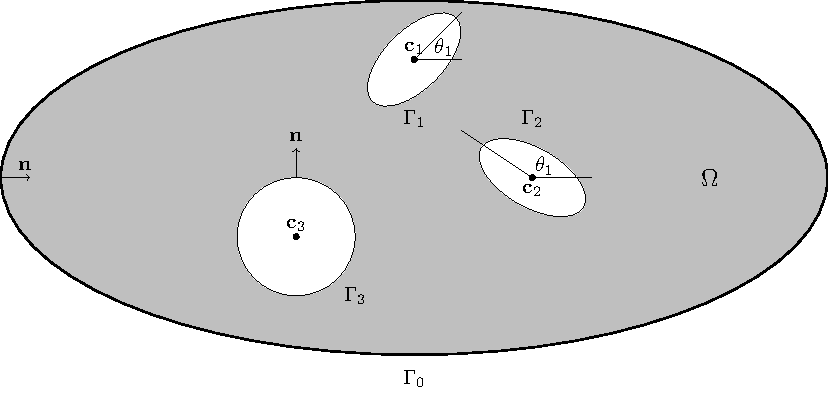
\includegraphics{figures/multiply_connected.pdf}
\end{center}
\caption{\label{fig:geomSchematic}A sketch of a bounded fluid domain
$\Omega$.  $\gamma_1$ and $\gamma_2$ enclose rigid particles, while
$\Gamma_1$ is a solid wall.  If $\Omega$ is unbounded,  $\Gamma_0$  is
not present.  The vector $\nn$ is the unit normal vector pointing out of
the fluid domain.}
\end{figure}

%%%%%%%%%%%%%%%%%%%%%%%%%%%%%%%%%%%%%%%%%%%%%%%%%%%%%%%%%%%%%%%%%%%%%%%%%%%%%%%
\subsection{Governing Equations}\label{sec:governing}

%We start by assuming that the fluid is governed by the incompressible
%Navier-Stokes equations 
%\begin{align*}
%  \rho\left(\pderiv{\uu}{t} + (\uu \cdot \grad) \uu \right) &= 
%    -\grad p + \mu \Delta \uu \qquad \xx\in\Omega,\\
%    \grad \cdot \uu &= 0 \qquad \xx\in\Omega,
%\end{align*}
%where $\uu$ is the velocity, $p$ is the pressure, $\rho$ is the fluid
%density, and $\mu$ is the fluid viscosity.  The equations are
%nondimensionalized in the standard method which results in the
%dimensionless Reynolds number.  

We are interested in small particles and slow velocities which renders
the Reynolds number small $\Re \ll 1$, and the fluid is governed by the
incompressible Stokes equations.  A Dirichlet boundary condition $\UU$
is imposed on the solid walls $\Gamma$, a no-slip boundary condition is
assumed for the rigid bodies $\gamma$, and the rigid bodies are assumed
to be force and torque free.  On each solid wall, there is a net force
and torque, $\FF^\Gamma_i$ and $L^\Gamma_i$, respectively, that it
applies to the fluid, and similar forces and torques are defined for
each rigid body, but these, for the time being, are assumed to be 0.
Therefore, the governing equations for $M_p$ particles suspended in a
bounded $M_w$-connected domain is
\begin{equation}
  \label{eqn:modelEquations}
  \begin{split}
  \mu \Delta \uu = \grad p, &\hspace{20pt} \xx \in \Omega, \gap
    &&\mbox{\em conservation of momentum,}\\
  \grad \cdot \uu = 0, &\hspace{20pt} \xx \in \Omega, \gap
    &&\mbox{\em conservation of mass,} \\
  \uu = \UU, &\hspace{20pt} \xx \in \Gamma, \gap 
    &&\mbox{\em wall velocity,} \\
  \uu = \uu^\tau_j + \omega_j(\xx-\cc^\gamma_j)^\perp,&\hspace{20pt} 
    \xx \in \gamma, \gap &&\mbox{\em no-slip on the particles,} \\
  \FF_j^\gamma = 0, &\hspace{20pt}j=1,\ldots,M_p, \gap 
    &&\mbox{\em force-free particles,} \\
  L_j^\gamma = 0, &\hspace{20pt}j=1,\ldots,M_p, \gap 
    &&\mbox{\em torque-free particles.}
  \end{split}
\end{equation}
Here, $\uu$ is the velocity, $p$ is the pressure, $\mu$ is the fluid
viscosity, $\uu^\tau_j$ and $\omega_j$ are the translational and
rotational velocities of rigid body $j$, respectively, and
$\FF_j^\gamma$ and $L_j^\gamma$ are the net force and torque of rigid
body $j$.  For the suspension of rigid bodies, the fluid viscosity sets
the time scale, and we assume it is one throughout the paper.  In the
case that the fluid domain is unbounded, the wall velocity equation is
replaced with the far-field condition
\begin{align*}
  \uu(\xx) = \uu_\infty(\xx), \quad |\xx| \rightarrow \infty.
\end{align*}
Then, given the rigid body translational and rotational velocities,
their centers and inclination angles $(\cc_j,\theta_j)$,
$j=1,\ldots,M_p$, satisfy
\begin{align}
\begin{split}
  \frac{d\cc_j}{dt} = \uu^\tau_j, \qquad 
  \frac{d\theta}{dt} = \omega_j.
\end{split}
\label{eqn:centersAngles}
\end{align}
Equations~\eqref{eqn:modelEquations} and~\eqref{eqn:centersAngles} govern
the dynamics of the rigid body suspensions, and their numerical solution
is a focus on this paper.

We have assumed that the rigid bodies are force- and torque-free.
However, as when two rigid bodies are brought sufficiently close
together, numerical errors can easily cause the rigid bodies to
unphysically intersect.  To avoid contact,  we will later relax the
force- and torque-free conditions to guarantee that numerical errors do
not cause rigid bodies do not come into unphysical contact.  This idea
is first described for vesicle suspensions by Lu et al.~\cite{Lu2017}
and we summarize the method in Section~\ref{sec:repulsion}.  


%%%%%%%%%%%%%%%%%%%%%%%%%%%%%%%%%%%%%%%%%%%%%%%%%%%%%%%%%%%%%%%%%%%%%%%%%%%%%%%
\subsection{Boundary Integral Equation Representation}
There exist many numerical methods for simulating the suspensions of
interfaces in a fluid by solving~\eqref{eqn:modelEquations} such as
level set methods~\cite{Dou2007}, immersed boundary methods~\cite{Mittal2005}, disipative particle dynamics~\cite{Pivkin2010}, smoothed particle hydrodynamics~\cite{Polfer2016}, or lattice Boltzmann
methods~\cite{Ladd1994a, Ladd1994b}. However, given that the fluid
equations are linear and the geometry mobile, we use a boundary integral
equation (BIE) formulation~\cite{Pozrikidis1992}.  BIEs have several
advantages including that only the interface has to be tracked, which
simplifies the representation of complex geometries, and high-order
discretizations are straightforward.  We now reformulate
equations~\eqref{eqn:modelEquations} as a BIE.

We start by formulating the incompressible Stokes equations in the
absence of rigid bodies.  The {\em double-layer potential} is the
convolution of the stresslet with an arbitrary density
function~\cite{Ladyzhenskaya1963, Pozrikidis1992},
\begin{align}
  \label{eqn:dlp}
  \uu(\xx) = \DD[\eeta](\xx) = \frac{1}{\pi}\int_{\Gamma}
  \frac{\rr\cdot\nn}{\rho^2}\frac{\rr \otimes \rr}{\rho^2}
  \eeta(\yy)~\text{d}s_{\yy}, \quad \xx \in \Omega,
\end{align}
where $\rr = \xx - \yy$, $\rho=|\rr|$, and $\eeta$ is an unknown density
function defined on $\bd\Omega$.  The double-layer
potential~\eqref{eqn:dlp} satisfies the incompressible Stokes equations,
and the Dirichlet boundary condition $\UU$ is also satisfied if
$\eeta$ satisfies~\cite{Pozrikidis1992}
%\begin{align*}
%  \lim_{\substack{\xx \rightarrow \xx_0 \\ \xx \in \Omega}}
%    \DD[\eeta](\xx) = \UU(\xx_0), \quad \xx_0 \in \Gamma,
%\end{align*}
%for $\eeta$.  When taking the limit, the singularity of the stresslet
%results in a jump~\cite{Pozrikidis1992}, and the density function must
%satisfy  
\begin{align}
  -\frac{1}{2} \eeta(\xx_0) + \DD[\eeta](\xx_0) = \UU(\xx_0), 
    \quad \xx_0 \in \Gamma.
  \label{eqn:secondKindBIE}
\end{align}
While the double-layer potential satisfies the incompressible Stokes
equations, it cannot represent all solutions of the incompressible
Stokes equations; in particular, it cannot represent rigid body motion.
This is rectified by introducing point forces and torques due to each
interior component of the geometry $\Gamma_j$~\cite{Power1987,
Power1993}, and the strengths of these forces and torques are related to
the density function.  By introducing the velocity fields due to a point
force (Stokeslet) and a point torque (rotlet), both centered at $\cc$,
\begin{align*}
  \mathbf{S}(\xx,\cc) = \frac{1}{4\pi}\left(-\log\rho\mathbf{I} + 
  \frac{\rr \otimes \rr}{\rho^2}\right), \quad \text{and} \quad
  \mathbf{R}(\xx,\cc) = \frac{\rr^\perp}{4\pi\rho^2},
\end{align*}
where $\rr = \xx - \cc$ and $\rho = |\rr|$.  Then, the second-kind
integral equation~\eqref{eqn:secondKindBIE} is replaced with the
completed second-kind BIE
\begin{equation}
  \label{eqn:completed_DLP}
  \begin{split}
  -\frac{1}{2}\eeta(\xx_0) + \DD[\eeta](\xx_0) + 
    \sum_{j=1}^{M_w} \left(\mathbf{S}(\xx,\cc^\Gamma_j)\FF^\Gamma_j + 
      \mathbf{R}(\xx,\cc^\Gamma_j)L^\Gamma_j\right) &= \UU(\xx_0),
      \quad &&\xx_0 \in \Gamma, \\
  \int_{\Gamma_j} \eeta~\text{d}s &= \FF^\Gamma_j, 
      &&j=1,\ldots,M_w, \\
  \int_{\Gamma_j} \eeta\cdot (\xx - \cc^\Gamma_j)^\perp~\text{d}s &=   
      L^\Gamma_j, &&j=1,\ldots,M_w.
  \end{split}
\end{equation}

We now introduce a suspension of rigid bodies $\gamma_j$,
$j=1,\ldots,M_p$.  Since the fluid boundary consists of both the solid
walls and rigid bodies, the limits of the integral of the double-layer
potential includes the rigid bodies and the solid walls.  Imposing the
no-slip boundary condition on the rigid bodies, a BIE formulation of the
suspension of rigid bodies governed by
equation~\eqref{eqn:modelEquations} is
\begin{subequations}
  \label{eqn:BIEformulation}
  \begin{align}
    \UU(\xx) &= -\frac{1}{2}\eeta(\xx) + \DD[\eeta](\xx) +
    \sum_{j=1}^{M_w} \left(\mathbf{S}(\xx,\cc^\Gamma_j)\FF^\Gamma_j + 
      \mathbf{R}(\xx,\cc^\Gamma_j)L^\Gamma_j\right)  \nonumber \\
&\hspace{96pt}+\sum_{j=1}^{M_p} \left(\mathbf{S}(\xx,\cc^\gamma_j)\FF^\gamma_j +
\mathbf{R}(\xx,\cc^\gamma_j)L^\gamma_j\right),
    \quad \xx \in \Gamma, \label{eqn:BIEformulation1} \\
  \uu^\tau_j + \omega_j(\xx - \cc_j^\gamma)^\perp &=
    -\frac{1}{2}\eeta(\xx) + \DD[\eeta](\xx) + 
    \sum_{j=1}^{M_w} \left(\mathbf{S}(\xx,\cc^\Gamma_j)\FF^\Gamma_j + 
      \mathbf{R}(\xx,\cc^\Gamma_j)L^\Gamma_j\right) \nonumber \\
&\hspace{96pt}+\sum_{j=1}^{M_p} \left(\mathbf{S}(\xx,\cc^\gamma_j)\FF^\gamma_j +
\mathbf{R}(\xx,\cc^\gamma_j)L^\gamma_j\right),
    \quad \xx \in \gamma, \label{eqn:BIEformulation2} \\
  \int_{\Gamma_j} \eeta~\text{d}s &= \FF^\Gamma_j, \quad
  \int_{\Gamma_j} \eeta\cdot (\xx - \cc^\Gamma_j)^\perp~\text{d}s =
  L^\Gamma_j, \quad j=1,\ldots,M_w, \label{eqn:BIEformulation3} \\
  \int_{\gamma_j} \eeta~\text{d}s &= \FF^\gamma_j, \quad
  \int_{\gamma_j} \eeta\cdot (\xx - \cc^\gamma_j)^\perp~\text{d}s =
  L^\gamma_j,\quad j=1,\ldots,M_p, \label{eqn:BIEformulation4} \\
  \FF^\gamma_j &= 0, \quad \L^\gamma_j = 0,\quad j=1,\ldots,M_p.
  \label{eqn:BIEformulation5}
\end{align}
\end{subequations}
Again, we have used the methodology of Power and
Miranda~\cite{Power1987, Power1993} to relate the strength of the
Stokeslets and rotlets of each rigid body to its density function.  The
BIE formulation~\eqref{eqn:BIEformulation} of the governing
equations~\eqref{eqn:modelEquations} consists of eight equations for
eight unknowns: the density function, net force, and net torque on the
solid walls and rigid bodies, and the translational and rotational
velocities.

While~\eqref{eqn:BIEformulation1} and~\eqref{eqn:BIEformulation2} are
both numerically desirable second-kind Fredholm integral equations
equations, equation~\eqref{eqn:BIEformulation1} has a rank one null
space because of the flux-free condition of the boundary data
$\UU$~\cite{Ladyzhenskaya1963}.  Following~\cite{Power1993}, this null
space is removed by adding the term 
\begin{align}
\label{eqn:N0_modification} 
  \mathcal{N}_0[\eeta](\xx) = \int_{\Gamma_0} 
    \nn(\xx)\otimes\nn(\yy)~\text{d}s(\yy)
\end{align}
to~\eqref{eqn:BIEformulation1}, but only for points $\xx \in \Gamma_0$.
Finally, if $\Omega$ is unbounded, there is no null space, and
the only modification to~\eqref{eqn:BIEformulation} is that
equation~\eqref{eqn:BIEformulation1} is removed and
equation~\eqref{eqn:BIEformulation2} has the background velocity
$\uu_\infty(\xx)$ added to the right hand side.


%%%%%%%%%%%%%%%%%%%%%%%%%%%%%%%%%%%%%%%%%%%%%%%%%%%%%%%%%%%%%%%%%%%%%%%%%%%%%%%
\subsection{A contact based repulsion force}
\label{sec:repulsion}
Exact solutions of the Stokes equations prohibit contact between force-
and torque-free particles in finite time.  Therefore, any contact
between rigid bodies is caused by numerical errors.  The two main
sources of error are the quadrature error---especially for nearly
touching rigid bodies---and time stepping error.  We address the
quadrature error using a combination of upsampling and
interpolation, and details of the method are described
in~\cite{Quaife2014}.  Time stepping have recently received more
attention, and methods that control stiffness~\cite{Quaife2014}, and use
adaptive time step sizes~\cite{Kropinski1999, Quaife2015,
Sorgentone2018}.  We describe time stepping methods in
Section~\ref{sec:temporal}.

%When evaluating a target point close to the boundary (as is
%necessary when two particles come close together) the kernel in the
%double layer potential becomes very sharply peaked and thus difficult to
%integrate accurately. Spatial and temporal adaptivity
%\cite{Kropinski1999}, special integration techniques \cite{Klockner2013,
%Ying2006} or asymptotic expansions of lubrication forces
%\cite{Mammoli2006} are all tools that can help, however even if we
%evaluate the double layer potential accurately, time stepping errors can
%still lead to contact. To keep computational costs reasonable we must
%turn to alternative approaches. 

%\begin{figure}[!h]\label{fig:collision_sketch}
%\begin{center}
%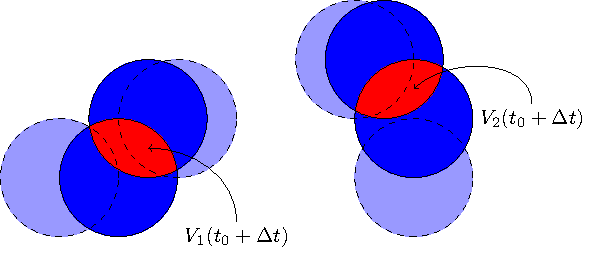
\includegraphics{figures/collisions.pdf}
%\end{center}
%\caption{Sketch of potential collisions.}
%\end{figure}

%Alternatively, repulsion forces can be added~\cite{Malhotra2018}, or
%the analytic solutions of the flow due to lubrication forces can be
%added to the dynamics~\cite{Mammoli2006}.  Unfortunately, repulsion
%forces often introduce non-linear stiffness that restricts the time step
%size, and using lubrication theory is difficult for particles of
%arbitrary geometry due to the complicated asymptotics needed.

We adopt the method of introducing an artificial force to avoid
collision.  There are many possible choices for the type of force. One
possibility is a Morse or Lennard-Jones potential that grows as a high
order polynomial as two particles approach~\cite{Flormann2017, Liu2006}. This has been shown to work for
dense suspensions, however the resulting ODEs become very stiff as the
separation between particles decreases, thus requiring smaller time
steps. Spring based models~\cite{Tsubota2006, Zhao2013, Kabacogulu2017}
have also been used to generate artificial repulsion forces, although
these models also introduce stiffness. One further disadvantage of these
methods is that neither approach explicitly guarantees no contact
between particles. If too large a time step is chosen collisions can
still occur. 

Instead, we apply a modification of the contact-aware method of Lu et
al.~\cite{Lu2017} where the choice of forces and torques guarantee that
each time step is collision-free.  We only summarize the method, but a
in-depth description is in~\cite{Lu2017}.  The method is based on the
variational form of the Stokes equations,
\begin{align}
  \min \int_{\Omega} \nabla\uu:\nabla\uu~\text{d}\Omega,
  \quad\text{ such that }\quad \nabla\cdot\uu = 0, 
  \quad \xx \in \Omega.
  \label{eqn:stokesEL}
\end{align} 
First, the space-time interference volume (STIV) is defined to be the
area in space-time swept out by the trajectory of two particles.  Then,
equation~\eqref{eqn:stokesEL} are supplemented with an additional
constraint that the STIV is negative (no contact).  By introducing
an additional Lagrange multiplier, $\lambda$, (the pressure is the other
Lagrange multiplier), the result is a body force that is restricted to
the rigid body boundaries.   Solving for $\lambda$ requires solving a
nonlinear complementary problem (NCP) which is solved iteratively using
a sequence of linear complementary problem (LCP) solves.

The NCP explicitly requires that the STIV is zero, meaning that there is
no contact.  Therefore, unlike most repulsion-based methods, the
contact-aware method guarantees that there is no collision.  However, it
is possible that the sequence of LCPs is not able to converge to a
solution of the NCP.  This stalling typically occurs if the interaction
between two bodies in close proximity is treated explicitly.  Therefore,
in Section~\ref{sec:temporal} we describe a new time stepping method
that allows for much closer contact without the contact algorithm
stalling.

%%%%%%%%%%%%%%%%%%%%%%%%%%%%%%%%%%%%%%%%%%%%%%%%%%%%%%%%%%%%%%%%%%%%%%%%%%%%%%%
%\begin{comment}
%\subsection{Avoiding Contact with STIV}
%Before discussing how collisions can be resolved, we first define a
%metric that measures collision.  This metric should track all pairwise
%collisions and detect if a two particles overlapped not only at the
%discrete time points, but at any time.  We let $\mathbf{V}(t)$ be a
%vector with size $\binom{M_p}{2}$ which is the total number of possible
%pairwise collisions.  $\mathbf{V}$ should be defined in such a way that
%it is 0 if no collisions have occurred, and if there is a collision, its
%value should quantify the amount of overlap.   Then, if there is a
%collision between two particles, the repulsion force should be chosen to
%scale with the magnitude of the corresponding entry of $\mathbf{V}$.
%There are several possible choices for $\mathbf{V}(t)$, the simplest
%being a signed distance between all points on all particles. We use the
%concept of {\em Space-Time Interference Volumes} (STIV) introduced by
%Harmon et al.~\cite{Harmon2011} and adapted for the suspension of
%deformable and rigid particles~\cite{Lu2017}. STIVs involve a time
%integral and are therefore more expensive to compute than other metrics
%(e.g. a signed distance). In most simulations however the cost of
%computing an STIV is dwarfed by the cost of the linear solves necessary
%to compute the velocities of the particles. The advantage of STIVs
%compared to simpler metrics is that under the assumption of ballistic
%motion they are able to detect collisions between two particles that
%pass completely through one another, i.e. it can detect that a collision
%has occurred even if the final candidate configuration is contact-free.
%
%%%%%%%%%%%%%%%%%%%%%%%%%%%%%%%%%%%%%%%%%%%%%%%%%%%%%%%%%%%%%%%%%%%%%%%%%%%%%%%%
%\subsection{Variational Formulation}
%The incompressible Stokes equations can be can be restated as a minimization
%problem. Consider the functional,
%\[ \mathcal{J}(\mathbf{u}) = \int_{\Omega} \nabla\mathbf{u}:\nabla\mathbf{u} -
%2\mathbf{f}\cdot\mathbf{u} ~\text{d}\Omega,\]
%and the associated constrained minimization problem,
%\[ \min \mathcal{J}(\mathbf{u}) ~:~ \nabla\cdot\mathbf{u} = 0 \text{ in
%}\Omega.\]
%Introducing $p$, a Lagrange multiplier for the incompressibility condition, we
%can construct a Lagrangian for this system,
%\begin{equation}\label{eq:lagrangian} \mathcal{L}(\mathbf{u},p) =
%\mathcal{J}(\mathbf{u}) - \int_{\Omega}
%2p\nabla\cdot\mathbf{u}~\text{d}\Omega.\end{equation}
%First order optimality (KKT) conditions for $\mathcal{L}(\mathbf{u},p)$
%recover the incompressible Stokes equations. For our problem, in
%addition to the incompressibility condition, we wish to enforce the
%constraint that the solution $\mathbf{u}$ at a time $t_0$ should not
%introduce collisions at time $t_0+\Delta t$, in other words
%$\mathbf{V}(t_0 + \Delta t) \geq \mathbf{0}$.  This constraint can be
%incorporated in the Lagrangian \eqref{eq:lagrangian} with the
%introduction of a Lagrange multiplier $\llambda$ with one component
%for each possible collision volume,
%\begin{equation}\label{eq:lagrangian2} \tilde{\mathcal{L}}(\mathbf{u},p,\lambda)=
%\mathcal{L}(\mathbf{u},p) + \pmb{\lambda} \cdot \mathbf{V}(t_0+\Delta
%t).\end{equation}
%First order optimality for \eqref{eq:lagrangian2} yields the Stokes equations
%with a modified forcing function,
%\begin{equation}\label{eq:stokes_mod}-\Delta \mathbf{u} + \nabla p = \mathbf{f}%+ \int_{\Omega}
%\text{d}_{\mathbf{u}} \mathbf{V}^T\pmb{\lambda}
%~\text{d}\Omega,\end{equation}
%subject to the constraints
%\[ \nabla\cdot\mathbf{u} =0, ~\mathbf{V}(t_0 + \Delta t) \geq 0,~\pmb{\lambda}
%\geq 0, ~ \pmb{\lambda}\cdot\mathbf{V}(t_0+\Delta t) = 0. \]
%
%The constraints on $\mathbf{V}$ and $\pmb{\lambda}$ can be combined into a
%single constraint,
%\begin{equation}\label{eq:ncp_constraint} \mathbf{V}(t_0 + \Delta t)\geq
%\mathbf{0} \perp \pmb{\lambda}\geq \mathbf{0}.\end{equation}
%
%\end{comment}
%%%%%%%%%%%%%%%%%%%%%%%%%%%%%%%%%%%%%%%%%%%%%%%%%%%%%%%%%%%%%%%%%%%%%%%%%%%%%%%


%%%%%%%%%%%%%%%%%%%%%%%%%%%%%%%%%%%%%%%%%%%%%%%%%%%%%%%%%%%%%%%%%%%%%%%%%%%%%%%%
%\begin{comment}
%\subsection{Complementary Problem}
%
%To compute the repulsion forces we must first compute $\pmb{\lambda}$ for each
%time step such that \eqref{eq:ncp_constraint} is satisfied.
%Consider particles suspended in a fluid in an ambient flow $\mathbf{u}_\infty$.
%This flow can be an imposed background flow or come from solid walls. In the
%later case this velocity field is computed by solving the appropriate resistance problem. In either
%case this flow can be expressed as the sum of a translational component $\mathbf{u}_{\infty}^\tau$,
%a rotational component $\omega_{\infty}$
%and a strain component $\mathbf{e}_{\infty}$,
%\[ \mathbf{u}_{\infty}(\mathbf{x}) = \mathbf{u}_{\infty}^\tau +
%\omega_\infty\times \mathbf{x} + \mathbf{e}_\infty \cdot\mathbf{x}.\]
%The translational and rotational velocity as well as the density
%function of a collection of particles can be computed from the force,
%torque and strain rate~\cite{Karrila1991},
%\begin{equation}\label{eq:mobility} \begin{bmatrix} \mathbf{u}_\infty^\tau -
%\mathbf{u}_\tau\\ \omega^\infty - \omega \\\pmb{\eta}\end{bmatrix} =
%\mathcal{M}\begin{bmatrix}\mathbf{F}\\\mathbf{L}\\\mathbf{e}_\infty\end{bmatrix},\end{equation}
%where $\mathcal{M}$ is the {\em mobility tensor} and depends only on the
%particle configuration $\mathbf{q}^0$ at some time $t^0$. Assuming the
%only force and torques acting on particles arises from repulsion forces,
%we can decompose \eqref{eq:mobility} as,
%\[ \begin{bmatrix} \mathbf{u}_\infty^\tau - \mathbf{u}_\tau\\ \omega^\infty -
%\omega \\\pmb{\eta}\end{bmatrix} =
%\mathcal{M}\begin{bmatrix}\mathbf{0}\\\mathbf{0}\\\mathbf{e}_\infty\end{bmatrix}+
%\mathcal{M}\begin{bmatrix}\mathbf{F}_c\\\mathbf{L}_c\\\mathbf{0}\end{bmatrix}.\]Once
%we solve for $\mathbf{u}_\tau$ and $\omega$ we can update the positions an
%dangles of each particle using an explicit Euler step. With an abuse of
%notation,
%this lets us express a candidate configuration $\mathbf{q}^{1}$ as,
%\[ \mathbf{q}^{1} = \mathbf{q}^n + \Delta
%t\left(\mathcal{M}\begin{bmatrix}\mathbf{0}\\\mathbf{0}\\\mathbf{e}_\infty\end{bmatrix}
%+
%\mathcal{M}\begin{bmatrix}\mathbf{F}_c\\\mathbf{L}_c\\\mathbf{0}\end{bmatrix}\right).\]
%
%This candidate configuration must satisfy the constraint
%\eqref{eq:ncp_constraint}, which we will rewrite to show the dependence of
%$\mathbf{V}$ on both $\mathbf{q}^0$ and $\mathbf{q}^{1}$,
%\begin{equation}\label{eq:ncp_new}\mathbf{V}(\mathbf{q}^0,\mathbf{q}^{1})\geq
%\mathbf{0}\perp \pmb{\lambda}^n\geq \mathbf{0} \Rightarrow
%\mathbf{V}\left(\mathbf{q}^0, \mathbf{q}^0 + \Delta
%t\left(\mathcal{M}\begin{bmatrix}\mathbf{0}\\\mathbf{0}\\\mathbf{e}_\infty\end{bmatrix}
%+
%\mathcal{M}\begin{bmatrix}\mathbf{F}_c\\\mathbf{L}_c\\\mathbf{0}\end{bmatrix}\right)\right)
%\geq \mathbf{0} \perp\pmb{\lambda}\geq \mathbf{0} .\end{equation}
%
%This is a nonlinear complementary problem (NCP). We can see this by explicitly
%including the dependence of $\mathbf{V}$ on $\pmb{\lambda}$,
%\[\mathbf{V}\left(\mathbf{q}^0, \mathbf{q}^0 + \Delta
%t\left(\mathcal{M}\begin{bmatrix}\mathbf{0}\\\mathbf{0}\\\mathbf{e}_\infty\end{bmatrix}
%+ \mathcal{M}\begin{bmatrix} \int_{\Gamma_k}
%\text{d}_\mathbf{u}\mathbf{V}^T\pmb{\lambda}~\text{d}s\\ \int_{\Gamma_k}
%\text{d}_\mathbf{u}\mathbf{V}^T\pmb{\lambda}\cdot(\mathbf{x}-\mathbf{c}_k)^\perp~\text{d}s
%\\\mathbf{0}\end{bmatrix}\right)\right) \geq \mathbf{0} \perp\pmb{\lambda}\geq
%\mathbf{0} .\]
%
%A first order linearization of this NCP turns it into a sequence of linear
%complementary problems (LCP). Starting from an initial guess for
%$\pmb{\lambda}$, $\pmb{\lambda}^0$ the following sequence should converge to the solution of
%\eqref{eq:ncp_new}:
%\begin{equation}\label{eq:lcp}\begin{aligned}
%\mathbf{V}\biggl(\mathbf{q}^0 + \Delta
%t\biggl(\mathcal{M}\begin{bmatrix}\mathbf{0}\\\mathbf{0}\\\mathbf{e}_\infty\end{bmatrix}
%&+ \mathcal{M}\begin{bmatrix} \int_{\Gamma_k}
%\text{d}_\mathbf{u}\mathbf{V}^T\pmb{\lambda}^\ell~\text{d}s\\ \int_{\Gamma_k}
%\text{d}_\mathbf{u}\mathbf{V}^T\pmb{\lambda}^\ell\cdot(\mathbf{x}-\mathbf{c}_k)^\perp~\text{d}s
%\\\mathbf{0}\end{bmatrix}\biggr)\biggr) \\
%&+ \Delta t \mathcal{M}\begin{bmatrix}\int_{\Gamma_k}
%\text{d}_\mathbf{u}\mathbf{V}^T\pmb{\lambda}^{\ell+1}~\text{d}s\\
%\int_{\Gamma_k}
%\text{d}_\mathbf{u}\mathbf{V}^T\pmb{\lambda}^{\ell+1}\cdot(\mathbf{x}-\mathbf{c}_k)^\perp~\text{d}s
%\\\mathbf{0}\end{bmatrix}\frac{\partial\mathbf{V}}{\partial \mathbf{q}^1} \geq
%\mathbf{0} \perp \pmb{\lambda}^{\ell+1} \geq
%\mathbf{0}.\end{aligned}\end{equation}
%
%The sequence \eqref{eq:lcp} will be solved at each time step. 
%\end{comment}
%%%%%%%%%%%%%%%%%%%%%%%%%%%%%%%%%%%%%%%%%%%%%%%%%%%%%%%%%%%%%%%%%%%%%%%
\subsection{Computing the Pressure and Stress}
To understand the rheological and statistical properties of suspensions
of rigid bodies, it is necessary to compute quantities such as the
pressure, stress, and energy dissipation.  In the BIE setting, computing
these quantities is a post-processing step, and they are 
computed with high-order accuracy using methods described in
Section~\ref{s:method}.

The pressure of the two-dimensional double-layer potential is given by\cite{Power1993}
\begin{align*}
  p(\xx) = \frac{1}{\pi}\int_{\partial\Omega}\frac{1}{\rho^2}\left(
\mathbf{I} - 2\frac{\rr \otimes \rr)\nn}{\rho^2}\right)\cdot\eeta~\text{d}s,
\qquad\xx\in\Omega.
\end{align*}
The pressure of a Stokeslet and rotlet can be easily computed,
and the pressure resulting from the completed double-layer potential
formulation for the velocity~\eqref{eqn:completed_DLP} is
\begin{align}
  \label{eqn:pressure} 
  p(\xx) = \frac{1}{\pi}\int_{\partial\Omega}\frac{1}{\rho^2}\left(
    \mathbf{I} - 2(\rr \otimes \rr)\nn\right)\cdot\eeta~\text{d}s +
  \sum_{i=1}^{M_w}
  \frac{\FF_i^\Gamma\cdot(\xx-\cc_i^\Gamma)}{2\pi|\xx-\cc_i^{\Gamma}|^2}
  + \sum_{i=1}^{M_p}
    \frac{\FF_i^\gamma\cdot(\xx-\cc_i^\gamma)}{2\pi|\xx-\cc_i^\gamma|^2}.
\end{align}

To compute the stress tensor
\begin{align*} 
\ssigma = -p \mathbf{I} + \left(\nabla \uu + (\nabla\uu)^\intercal\right), \qquad
\xx\in\Omega,
\end{align*}
we start by using the layer potential representation of the
pressure~\eqref{eqn:pressure}.  Then, the viscous stress tensor is
determined by computing the Jacobian of the double-layer
potential~\eqref{eqn:dlp} and the Stokeslets and rotlets to form
\begin{align}
  \label{eqn:stress}
  \ssigma = \ssigma_{\eeta} + \ssigma_{S} + \ssigma_{R},
\end{align}
where
\begin{align*}
  \ssigma_{\eeta}(\xx) &= \frac{1}{\pi}\int_{\partial\Omega}\left( 
    \frac{\nn\cdot\eeta}{\rho^2}\mathbf{I} 
    -8\frac{(\rr\cdot\nn)(\rr\cdot\eeta)(\rr\otimes\rr)}{\rho^6} 
    +\frac{(\rr\cdot\nn)(\rr\otimes\eeta + \eeta\otimes\rr)}{\rho^4} 
+ \frac{(\rr\cdot\eeta)(\rr\otimes\nn +
\nn\otimes\rr)}{\rho^4}\right)\text{d}s,\\
  \ssigma_S(\xx) &= -\sum_{i=1}^{M_w} 
    \frac{\FF_i^\Gamma\cdot(\xx - \cc_i^\Gamma)}{\pi|\xx-\cc_i^\Gamma|^2}
        (\xx - \cc_i^\Gamma)\otimes(\xx - \cc_i^\Gamma)  -
    \sum_{i=1}^{M_p}
    \frac{\FF_i^\gamma\cdot(\xx - \cc_i^\gamma)}{\pi|\xx-\cc_i^\gamma|^2}
        (\xx-\cc_i^\gamma )\otimes(\xx-\cc_i^\gamma),\\
\ssigma_R(\xx) &= -\sum_{i=1}^{M_w} \frac{L_i^\Gamma}{2\pi|\xx-\cc_i^\Gamma|^2}
((\xx-\cc_i^\Gamma)\otimes(\xx-\cc_i^\Gamma)^\perp +
    (\xx-\cc_i^\gamma)^\perp\otimes(\xx-\cc_i^\gamma))  \\
\qquad&-\sum_{i=1}^{M_p}
\frac{L_i^\gamma}{2\pi|\xx-\cc_i^\gamma|^2}
    ((\xx-\cc_i^\gamma )\otimes(\xx-\cc_i^\gamma)^\perp + 
    (\xx-\cc_i^\gamma)^\perp\otimes(\xx-\cc_i^\gamma)).
\end{align*}

These expressions hold inside $\Omega$. On the boundary there is a jump in the pressure and stress, as reported in \cite{Quaife2014}.
Using the divergence theorem we can compute quantities like the volume average stress by computing only boundary integrals~\cite{Pozrikidis1992}. 
		
%%%%%%%%%%%%%%%%%%%%%%%%%%%%%%%%%%%%%%%%%%%%%%%%%%%%%%%%%%%%%%%%%%%%%%%
\section{Numerical Methods\label{s:method}} 

To compute rheological statistics, simulations must be run to a long horizon. With the goal of performing such long-time simulations of dense
suspensions, appropriate numerical methods must be employed.  To achieve
high-order accuracy, the spatial grid is resolved with spectral accuracy
(Section~\ref{sec:spatial}), and stability is achieved by using implicit
interactions in the time integrator and adaptive time stepping (Section~\ref{sec:temporal}). The computational cost is managed
with the fast multipole method
\cite{Greenbaum1992} and a
block-diagonal preconditioner.


%%%%%%%%%%%%%%%%%%%%%%%%%%%%%%%%%%%%%%%%%%%%%%%%%%%%%%%%%%%%%%%%%%%%%%%
\subsection{Spatial Discretization}\label{sec:spatial}

All the integral equations are discretized
with a Nystr\"om  methods, and interactions between nearly touching
interfaces is resolved with a near-singular integration scheme. By using
these methods, spectral accuracy can be achieved for long time horizons
with optimal complexity.

For particles that are in near-contact the near singular
integration scheme described in~\cite{Quaife2014, Ying2006} is used.

Let $\xx(\alpha)$ be a parameterization of a rigid body or a solid
wall which is represented with $N_p$ or $N_w$ Fourier modes. We can represent
smooth functions defined on this curve using a
Fourier series as
\begin{align}
  f(\alpha) = f(\xx(\alpha)) = \sum_{k \in \ZZ} \hat{f}_k e^{ik\alpha}.
\end{align}
The FFT is used to compute $\hat{f}$, and all derivatives are computed
with this Fourier series so that spectral accuracy is achieved.

The double-layer potentials in~\eqref{eqn:BIEformulation} are
discretized with a Nystr\"om method.  Because the kernels are smooth,
the trapezoid rule guarantees spectral accuracy~\cite{Trefethan2014}.
Equations~\eqref{eqn:BIEformulation}  are discretized as
\begin{equation*}
  \begin{aligned}
  \UU(\xx_i) = -\frac{1}{2}\eeta(\xx_i) + 
  \sum_{k=1}^{N} K(\xx_i,\xx_k) \eeta(\xx_k) \Delta s_k
    &+ \sum_{j=1}^{M_p} \left(\mathbf{S}(\xx_i,\cc^\gamma_j)\FF_j +
    \mathbf{R}(\xx_i,\dd_j)L_j\right)  \\
    &+ \sum_{j=1}^{M_w} \left(\mathbf{S}(\xx_i,\cc^\Gamma_j)\FF_j +
    \mathbf{R}(\xx_i,\cc^\Gamma_j)\L_j\right),
  \end{aligned}
\end{equation*}
\begin{equation*}
  \begin{aligned}
\uu^\tau_j + \omega_j(\xx_i - \cc^\gamma_j)^\perp = -\frac{1}{2}\eeta(\xx_i) +
\sum_{k=1}^{N} K(\xx_i,\xx_k) \eeta(\xx_k) \Delta s_k
    &+ \sum_{j=1}^{M_p} \left(\mathbf{S}(\xx_i,\cc^\gamma_j)\FF_j +
    \mathbf{R}(\xx_i,\dd_j)L_j\right)  \\
    &+ \sum_{j=1}^{M_w} \left(\mathbf{S}(\xx_i,\cc^\Gamma_j)\FF_j +
    \mathbf{R}(\xx_i,\cc^\Gamma_j)\L_j\right),
  \end{aligned}
\end{equation*}
where $N = M_w N_w + M_p N_p$ is the total number of discretization
points and
\begin{align*}
  K(\xx,\yy) = \frac{1}{\pi} \frac{\rr \cdot \nn}{\rho^2} 
               \frac{\rr \otimes \rr}{\rho^2}
\end{align*}
is the kernel of the double-layer potential.
 For the diagonal entries, we use the limiting value of $K$
\begin{align*}
  \lim_{\substack{\yy \rightarrow \xx \\ \yy \in \bd\Omega}} 
    K(\xx,\yy) = \frac{\kappa}{2\pi}\tt\otimes\tt,
    \quad \xx \in \bd\Omega,
\end{align*}
where $\kappa(\xx)$ is the curvature and $\tt(\xx)$ is the tangent
vector of $\bd\Omega$ at $\xx$.

The trapezoid rule achieves spectral accuracy when both the source
points $\yy$ and the target point $\xx$ are on the same solid wall
$\Gamma_k$ or rigid particle $\gamma_k$.  However, when the target point
is on a different body, the accuracy of the trapezoid rule can
deteriorate which leads to instabilities.  This increase in error
happens when the target point is close to the source points, but not on
the same body as the source points.  To resolve this issue, an algorithm
for near-singular integration method must be employed.  There are now
several methods for near-singular integration including
regularizations~\cite{Beale2001}, quadrature by
expansion~\cite{Klockner2013}, barycentric
interpolation~\cite{Barnett2015}, and panel-based
quadrature~\cite{Helsing2008}.  In this work, we use an interpolation
based scheme~\cite{Ying2006} which has been used for other
two-dimensional suspensions.  To compute the pressure and stress, odd-even integration with singularity subtraction is used.~\cite{Quaife2014}.

Once all of the equations in~\eqref{eqn:BIEformulation} are discretized
using the above described quadrature rules, the result is a dense $N
\times N$ linear system.  Since this linear system is the discretization
of a second-kind integral equation, GMRES~\cite{Saad1986} converges in a
mesh-independent number of iterations~\cite{Campbell1996}.  Since GMRES
only requires matrix-vector multiplications, the algorithmic cost per
time step is proportional to the cost of doing a single matrix-vector
multiply.
\todo[inline]{Discuss our preconditioner here?}


%%%%%%%%%%%%%%%%%%%%%%%%%%%%%%%%%%%%%%%%%%%%%%%%%%%%%%%%%%%%%%%%%%%%%%%
\subsection{Time Stepping Methods}
\label{sec:temporal}

We use a Lagrangian formulation where we track the centers
$\cc_i^\gamma$ and orientations $\theta_i$ of each rigid body
$\gamma_i$. Given a suspension of rigid
bodies,~\eqref{eqn:BIEformulation} is solved for the translational and
rotational velocities of each body. Then, the position and angle of each
particle are updated according to the ODEs,
\begin{align*}
  \frac{\text{d}}{\text{d}t}\mathbf{c}_k = \mathbf{u}^\tau_k, \qquad
  \frac{\text{d}}{\text{d}t}\theta_k =\omega_k.
\end{align*}
The ODEs are advanced in time using an explicit Euler step
\begin{align*}
  \cc_k^{N+1} &= \cc_k^N + \Delta t \left(\uu_k^\tau\right)^N, \\
  \theta_k^{N+1} &= \theta_k^N + \Delta t \left(\omega_k\right)^N.
\end{align*}
This low cost first-order time stepper is justifiable since we are
not interested in accurate particle trajectories, but rather are
interested in statistical quantities of bulk quantities related to the
suspension over large amounts of parameter values.

The stability of the method is depends strongly on the method used to
solve~\eqref{eqn:BIEformulation} for the translational and angular
velocities $\uu_j$ and $\omega_j$. If the numerical error of the
computed velocity is too large, unphysical contact will occur and
which STIV will attempt to resolve.  However, if large errors are caused
by interactions of bodies that are closer than the minimum separation
distance, then these errors will not be resolved by STIV unless a very
small time step is taken.  Therefore, if simulations result in nearly
touching bodies, such as in dense concentrations, the it is important to
use a time stepping method that allows for small minimum separations.

The leading source of stiffness for a particular rigid body
is the velocity field induced by the body itself. This leading source of
stiffness is typically resolved by using the {\em locally implicit}
discretization
\begin{align*}
  \DD[\eeta](\xx) \approx \DD^{n}[\eeta^{N+1}](\xx) +
  \DD^{n}[\eeta^N](\xx),
\end{align*}
where the superscript on the layer potential $\DD$ means that the layer
potential is defined in terms of the geometry at time step $n$.  A
secondary source of stiffness is caused by nearly touching bodies.  This
can be resolved by treating not only the self-interactions  implicitly,
but also treating the interactions between different bodies implicitly.
This method is the {\em globally implicit} discretization
\begin{align*}
  \DD[\eeta](\xx) \approx \DD^{N}[\eeta_{N+1}](\xx) +
  \DD^{N}[\eeta^{N+1}](\xx),
\end{align*}



While the interactions between
different bodies can be treated explicitly or implicitly, the layer
potential will always be discretized explicitly. By this we mean that
the density function $\eeta$ at time step $N$ will be discretized on the
body configuration at time step $N$.  In the original work of Lu et
al.~\cite{Lu2017}, they use a semi-implicit method where the interaction
between a rigid body and itself are treated implicitly, and all other
interactions are treated explicitly.  For example, in the governing
equation for the rigid bodies~\eqref{eqn:BIEformulation2}, double-layer
potential terms is discretized as
\begin{align}
 \DD[\eeta^{N+1}](\xx_j) \approx
  \DD[\eeta^{N+1}_{k_0}](\xx_j) + 
  \sum_{\substack{k=1 \\ k \neq k_0}}^{M_p} \DD[\eeta^{N}_k](\xx_j),
  \label{eqn:BlockImplicit}
\end{align}
where $\xx_j$ is on body $k_0$, the superscript denotes the time
step, and $\DD$ is discretized on the configuration at time step $N$. The interaction between the
rigid bodies and the solid walls'
density function, Stokeslets, and rotlets are also discretized
explicitly.  The advantage of this discretization is that it results in
a block-diagonal matrix structure that can be solved efficiently by using a block-diagonal
preconditioner. However, by allowing
larger interactions between different bodies, stiffness is introduced
and a smaller time step must be taken. 

Similar to the methodology
outline described for vesicle suspensions~\cite{Quaife2014}, we instead
change the fluid solver so that large time steps can still be taken
without introducing stiffness.  In particular, with the same setup
described in~\eqref{eqn:BlockImplicit}, we discretize the fluid
equations as
\begin{align}
  \DD[\eeta^{N+1}](\xx_j) = 
  \sum_{k=1}^{M_p} \DD[\eeta^{N+1}_k](\xx_j).
  \label{eqn:SemiImplicit}
\end{align}
Equation~\eqref{eqn:SemiImplicit} is no longer block-diagonal and requires additional computational
resources. In particular
interactions between different bodies must be computed at every
iteration rather than once per time step (to form the right hand side).
However, as was observed for dense vesicle suspensions~\cite{Quaife2014, Rahimian2015} this
additional cost is offset by the
excessively small time step that is required if the fluid
solver~\eqref{eqn:BlockImplicit} is used.  Moreover, as we will see in
the Results section, it is possible that if the buffer region is
sufficiently small and the suspension is sufficiently dense,
then~\eqref{eqn:BlockImplicit} is unstable for time step sizes that vary
over several orders of magnitude.

\subsection{Contact Resolution}

From an algorithmic point of view, contact resolution starts by
advancing the force- and torque-free particles from time $t$ to $t +
\Delta t$ according to equation~\eqref{eqn:centersAngles} where the
translational and angular velocities satisfy~\eqref{eqn:BIEformulation2}.
Next, collision detection is performed.  However, instead of requiring
that the bodies are contact-free, we make the additional restriction
that the minimum separation distance is greater than some user-specified
tolerance.  Finally, based on the amount of overlap that occurs,
artificial forces and torques are added to the bodies, and the governing
equations~\eqref{eqn:BIEformulation} are resolved, except that forces
and torques are included in equation~\eqref{eqn:BIEformulation5}.  

\begin{comment}
To
find the amount of overlap, the space-time interference volume
(STIV)~\cite{Harmon2011} based on a linear trajectory of the rigid
bodies is used. Once the new candidate solution is computed, the
algorithm is repeated until it converges to a contact-free
configuration.
\end{comment}

%At each time step $t^n$ the Stokes equations are solved and the
%particles are advanced to a candidate configuration at $t^{n+1}$.  Using
%a linear interpolant, we check if any collisions occurred in the
%interval $[t^n,t^{n+1}]$.  If the time step is contact-free, the
%candidate configuration is accepted.  If contact is detected, the
%candidate solution is rejected and we resolve
%equations~\eqref{eqn:BIEformulation}, but with artificial repulsion
%forces $\FF^\gamma_j$ and torques $L^\gamma_j$ that are chosen to try
%and avoid contact.  This lets us form a new candidate configuration.
%This process is repeated until we end up with a contact-free
%configuration.


As detailed in~\cite{Lu2017, Harmon2011}, space-time interference
volumes (STIV) offer a metric to quantify collision volumes. One
advantage of STIVs over other collision detection methods, such as a
signed distance, is that STIVs involve a time integral and can detect
collisions even if the final configuration is contact-free. Thus, even
if one particle passes completely through another, using STIVs we can
compute a contact volume and its response to changes in the velocity of
the particles.

Moreover, by including STIV with a sufficiently large buffer
region (on the order of an arclength term), the stiffness introduced by
interactions between different bodies is avoided. 


\subsection{Balancing Repulsion Forces}

%\begin{comment}
%The addition of a forcing term to the right hand side of the Stokes equations
%would normally lead to a volume integral. However, in this case since
%$\text{d}_{\mathbf{u}} V$ can be non-zero only on the boundary, we can capture
%the repulsion force by adding a net force and torque to each particle or wall as needed. The net
%force $\mathbf{F}^k_p$ and torque $L^k_p$ are given by,
%\[ \mathbf{F}^k_p = \int_{\Gamma_k}
%\text{d}_\mathbf{u}V^T\pmb{\lambda}~\text{d}s, \qquad L_p^k = \int_{\Gamma_k}
%\text{d}_\mathbf{u}V^T\pmb{\lambda}\cdot(\mathbf{x}-\mathbf{c}_k)^\perp~\text{d}s.\]
%\end{comment}

Physically we expect that any repulsion force exerted by one particle on another is balanced by an
equal and opposite repulsion force from the second particle.
In this way the net force in the system coming from repulsion forces is always
zero, i.e.
\begin{equation*}
	\sum\limits_{j=1}^{M_p} \FF^\gamma_j = \mathbf{0}.
\end{equation*}
This is particularly important for unbounded domains, as for planar flow Stokes
paradox says that only force-free configurations have bounded solutions at
infinity \cite{Power1993, Pozrikidis1992}.

If only two particles are in contact, the symmetry of the STIV ensures that the
net force is zero. However, if one particle is in contact with more than one
particle, then due to the scaling of the magnitudes of the forces, the net force may be nonzero. In
this case the repulsion forces may need to be balanced manually. To do this, we group all particles
that are in contact into distinct clusters.
For each cluster, the particle that is in contact with the most other particles
(to break ties, the particle with the largest repulsion force in magnitude) is
given a net force that balances all other particles in the
cluster. Whenever a the force on a particle is scaled the torque on that
particle is scaled by the same amount.

\subsection{Temporal Adaptivity}

The NCP solver is quite sensitive to the initial configuration.
Occasionally it may take an unfeasible amount of LCP iterations to
converge. To avoid this we adopt a heuristic adaptive time stepping
scheme. Once the number of LCP iterations crosses a threshold, if we
find the STIV volume is not decreasing fast enough we abort the time
step and restart it with a time step size of $\Delta t/2$. If, conversely, the NCP
converges in a small number of LCP iterations, we increase $\Delta t$
by a factor of $1.5$.


\begin{comment}
%%%%%%%%%%%%%%%%%%%%%%%%%%%%%%%%%%%%%%%%%%%%%%%%%%%%%%%%%%%%%%%%%%%%%%%
\subsection{Fast Summation and Preconditioning}
\todo[inline]{Do we describe how the preconditioner is updated by simply
rotating?}
After discretizing~\eqref{eqn:bieformulation1}
and~\eqref{eqn:bieformulation2} using the Nystr\"om method, dense linear
systems need to be solved.  The discretized system is solved with
GRMES~\cite{Saad1986}, and since these are both second-kind Fredholm
integral equations, the number of required GMRES iteartions is
independent of the resolution~\cite{cam-ips-kel-mey-xue1996}.

with a block diagonal preconditioner and
accelerated using the fast multipole method \cite{Greengard1987}.  Since
the linear system arises from a second kind Fredholm equation the
condition number of the matrix is bounded and does not increase with
finer resolution. The number of GMRES iterations is therefore mesh
resolution independent. This leads to a solver that is $O(n)$, where $n$
is the number of mesh points. 

The matrices described in \eqref{eq:vel_walls} and
\eqref{eq:vel_particles} are full. They can be made block-diagonal by
treating inter-particle interactions explicitly and moving them to the
right hand side. This is termed {\em locally implicit} and is described
in \cite{Lu2017}. For dense suspensions however this type of time
stepping can lead to instabilities as particles become tightly packed. 
\end{comment}
\begin{comment}
\begin{algorithm}
	 \SetKwInOut{Input}{Input}
    	\SetKwInOut{Output}{Output}

  	  \underline{Collision free time stepper}\;
\Input{collision free configuration $\mathbf{q}^0$, time step size $\Delta t$}
\Output{collision free configuration $\mathbf{q}^1$ }
	 $\mathbf{u}^* \gets \mathbf{A}(\mathbf{q}^0,\mathbf{0},\mathbf{0})$\;
	$\mathbf{q}^* \gets \mathbf{q}^0 + \Delta t \mathbf{u}^*$\;
	Compute $\mathbf{V}(\mathbf{q}^0,\mathbf{q}^*)$, $\text{d}_u\mathbf{V}$\;
	\While {$\mathbf{V} < \mathbf{0}$}
	{
		$\llambda \gets$ LCP\_solve($\text{d}_{\mathbf{u}}\mathbf{V}$)\;
$\mathbf{F}_k \gets \int_{\Gamma_k}
\text{d}_{\mathbf{u}}\mathbf{V}^T\llambda~\text{d}s$\;
$L_k \gets \int_{\Gamma_k}
\text{d}_{\mathbf{u}}\mathbf{V}^T\llambda\cdot(\mathbf{x}-\mathbf{c}_k)^\perp~\text{d}s$\;
		$\mathbf{u}^* \gets \mathbf{A}(\mathbf{q}^0,\mathbf{F}_k,\mathbf{L}_k)$\;
		$\mathbf{q}^* \gets \mathbf{q}^0 + \Delta t \mathbf{u}^*$\;
		Compute $\mathbf{V}(\mathbf{q}^0,\mathbf{q}^*)$, $\text{d}_u\mathbf{V}$\;
	}
\end{algorithm}
\end{comment}

%%%%%%%%%%%%%%%%%%%%%%%%%%%%%%%%%%%%%%%%%%%%%%%%%%%%%%%%%%%%%%%%%%%%%%%
\section{Results\label{s:results}} 
We use our new time stepping method to simulate bounded and unbounded
suspensions of two-dimensional rigid bodies in a viscous fluid.  The
main parameters are the minimum separation distance $\delta$, the number
of discretization points of each body, $N_p$, and each solid wall,
$N_w$, and the initial time step size $\Delta t$. We perform convergence
studies and investigate the effect loss of reversibility caused by the
STIV algorithm.  To further demonstrate the consequence of STIV, we
include plots of streamlines that cross whenever the collision detection
algorithm is applied.  The particular experiments we perform are now
summarized.
\begin{itemize}
  \item {\bf Shear Flow}: We consider the standard problem of two
  identical rigid circles in the shear flow $\uu = (y,0)$ with the left
  body slightly elevated from the right body.  We report similar results
  to those presented in~\cite{Lu2017}, but we are able to take smaller
  initial displacements and minimum separation distances.  The contact
  algorithm breaks the reversibility of the flow, and this effect is
  illustrated and quantified.

  \item {\bf Taylor-Green Flow}: We simulate a concentrated suspension
  of 48 rigid ellipses in an unbounded Taylor-Green flow. At the
  prescribed separation distance, our new time stepping method is able
  to stably reach the time horizon, while the locally semi-implicit time
  integrator proposed by Lu et al.~\cite{Lu2017} results in the STIV
  algorithm stalling, even with $\Delta t = 10^{-8}$.

  \item {\bf Porous Monolayer Injection}: We consider a suspension of
  confined rigid circular bodies motivated by an experiment by MacMinn
  et al.~\cite{MacMinn2015}.  The geometry is an annulus with an inflow
  at the inner boundary and an outflow at the outer boundary.  We again
  examine the effect STIV on the reversibility of the flow, and compute
  the shear strain rate and make qualitative comparisons to results for
  deformable bodies~\cite{MacMinn2015}.

  \item {\bf Taylor-Couette Flow}: With the ability to do high area
  fraction suspensions without imposing a large non-physical minimum
  separation distance, we simulate rigid bodies of varying aspect ratios
  inside a Taylor-Couette device.  We examine the effect of the rigid
  body shape and area fraction on the effective viscosity and the
  alignment angles.
\end{itemize}



%%%%%%%%%%%%%%%%%%%%%%%%%%%%%%%%%%%%%%%%%%%%%%%%%%%%%%%%%%%%%%%%%%%%%%%
\subsection{Shear Flow}
We start by repeating an experiment~\cite{Lu2017} to compare our new
globally implicit time integrator with the locally implicit version.
The initial condition is two rigid circles arranged placed symmetrically
about the origin, but with the left body slightly elevated.  In the
shear flow ${\uu}(\xx) = (y,0)$, the bodies approach, come into near
contact, and then separate.  Each particle is discretized with $N=32$
points and the arc length spacing $h = 2\pi/32 \approx 0.196$.  

As a first experiment, we set $\Delta t = 0.4$ and $\delta = 0$.  Then,
the new method globally implicit method successfully reaches the time
horizon without requiring a repulsion force.  However, with the same
$\Delta t$, the local explicit time stepping results in a collision
between the particles, so the collision algorithm is required to reach
the time horizon.  Alternatively, the time step size can be reduced,
but, as we will see, for sufficiently dense suspensions, even an
excessively small time step size results in collisions.

In Figure~\ref{fig:shear_experiment}, we investigate the effect of the
minimum separation distance on the position of the rigid bodies.  As reported in \cite{Lu2017}, as the minimum separation  distance  $\delta$ between particles decreases the excess vertical displacement goes to zero. Once $\delta$ is large enough for the constraint to be active, the excess displacement looks to scale linearly with $\delta$.

\begin{figure}[!h]
  \begin{center}
    \includegraphics{figures/shear_setup1.pdf}
    \begin{tabular}{c c}
      \includegraphics{figures/shear_displacement1.pdf} &
      \includegraphics{figures/separation_displacement1.pdf}
    \end{tabular}
  \end{center}
\caption{\label{fig:shear_experiment} Shear experiment. Top: The initial
setup and trajectories of the left body.   Bottom left: The trajectory
of the left particle for varying minimum separation distances.  Bottom
right: The effect of the minimum separation distance $\delta$ on the
final vertical displacement of the left particle initially on the left.}
\end{figure}

We next investigate the effect of the collision algorithm on the time
reversibility of the flow. We reverse the shear direction at $t=10$ and
measure the error between the particle's center at $t=0$ and $t=20$.
The results for various values of $\delta$ are in
Table~\ref{tab:reverse}. We achieve identical first-order accuracy in
the reversibility of the flow for $\delta = 0$ (no contact constraint)
and $\delta=h$.  This is expected since we have applied a first-order
Euler method, and the contact algorithm is not required for $\delta =
h$.  For $\delta \geq 2h$, when the particles first come into contact,
they are deflected onto contact-free streamlines.  When the flow is
reversed, the particles again pass one another, but they are now on
contact-free streamlines, so the initial deflection is not reversed.
The error in the reversibility is the sum of the time stepping error and
the error from deflecting the bodies in the contact algorithm.  This is
demonstrated in Table~\ref{tab:reverse} since a smaller time step size
does not decrease the error in reversibility, indicating that error
caused by the contact algorithm dominates.

This break in reversibility is further demonstrated by examining
individual streamlines.  In Figure~\ref{fig:shear_cross}, we compute the
streamline of the left particle for three different initial placements.
Before the particles approach, the streamlines behave as expected---they
do not cross.  However, the contact algorithm is applied to the blue
streamline, and this has the effect of allowing the streamlines to
cross.

The effect of the contact force on the streamlines is shown in Figure
\ref{fig:shear_cross}. Keeping the minimum separation fixed at $\delta =
3h$, we vary the initial $y$ coordinate of the left particle. If the
initial $y$ coordinate is high enough, no repulsion force is needed to
prevent the particles coming within $\delta$ of each other. Once a
repulsion force is added however, the particle jumps to a different
streamline.

\begin{figure}[!h]
\begin{center}
\includegraphics{figures/shear_streamlines_cross.pdf}
\end{center}
\caption{Repulsion forces causes streamlines to cross. Keeping the
minimum separation fixed at $\delta=3h$, we vary the starting $y$
location of the left particle. The teal and red streamlines do not
require a repulsion force to enforce the minimum separation between the
particles, but the blue streamline does. Once the contact algorithm is
applied, the blue streamline crosses the other streamlines (middle
inset). This crossing of the streamlines breaks the reversibility of the
simulation.}\label{fig:shear_cross}
\end{figure}

\begin{table}[!h]
\begin{center}
\begin{tabular}{c| c c c c c}
$ $ & & & $\Delta t$ & &\\
$\delta$ & $4\e{-2}$ &$ 2\e{-2}$ & $1\e{-2}$ & $5\e{-3}$ & $2.5\e{-3}$\\
\hline
0 & $1.35\e{-1}$ & $7.32\e{-2}$ & $3.74\e{-2}$ & $2.00\e{-2}$ & $1.01\e{-2}$\\
$h$ & $1.35\e{-1}$ & $7.32\e{-2}$ & $3.74\e{-2}$ & $2.00\e{-2}$ & $1.01\e{-2}$\\
$2h$ & $1.88\e{-1}$ & $1.41\e{-1}$ & $1.17\e{-1}$ & $1.08\e{-1}$ &
$1.02\e{-1}$\\
$2.25h$ & $2.55\e{-1}$ & $2.08\e{-1}$ & $1.87\e{-1}$ & $1.78\e{-1}$ &
$1.73\e{-1}$\\
$2.50h$ & $3.05\e{-1}$ & $2.69\e{-1}$ & $2.52\e{-1}$ & $2.45\e{-1}$ &
$2.40\e{-1}$\\
$2.75h$ & $3.64\e{-1}$ & $3.31\e{-1}$ & $3.13\e{-1}$ & $3.07\e{-1}$ &
$3.03\e{-1}$\\
$3.00h$ & $4.12\e{-1}$ & $3.88\e{-1}$ & $3.72\e{-1}$ & $3.67\e{-1}$ &
$3.63\e{-1}$
\end{tabular}
\end{center}
\caption{A study of time reversibility of the shear flow example. At
$t=10$, the flow direction is reversed and we calculate the relative
error in the initial and final positions. When the collision constraint
is active and force is needed to keep the particles apart the error in
the reversibility is dominated by the contact
algorithm.}\label{tab:reverse}
\end{table}

\subsection{Taylor-Green}

For planar flows, we can separate suspensions into dilute and
concentrated regimes by comparing the number of particles per unit area,
$\nu$, to the average particle length $\ell$. If $\nu < 1/\ell^2$, then
we are in the dilute regime, otherwise we are in the concentrated regime
(in 2D planar suspensions, unlike 3D suspensions, there is no concept of
semi-dilute regimes).  We next consider the suspension of 75 rigid
particles in the Taylor-Green flow $\mathbf{u}^\infty = (\cos(x)\sin(y),
-\sin(x)\cos(y))$.  The number of particles per unit area is $\nu
\approx 3.1$ which is greater than $1/\ell^2=1.108$.  Therefore, this
suspension is well within the concentrated regime. 

We discretize the particles with $N=32$ points and select the minimum
separation distance $\delta=0.05h$. Snapshots of the simulation are
shown in Figure \ref{fig:taylor_green}.  In this concentrated
suspension, the particles come into contact much more frequently.  If
the interactions between these nearly touching bodies are treated
explicitly, this leads to stiffness.  Our time stepper controls this
stiffness by treating these interactions implicitly, and the simulation
successfully reaches the time horizon.  We performed the same
simulation, but with the locally implicit time stepping
method~\cite{Lu2017}.  Because of the near-contact, smaller time step
sizes must be taken.  We took time step sizes as small as $10^{-8}$, and
the method was not able to successfully reach the time horizon.  This
exact behavior has also been observed for vesicle
suspensions~\cite{Quaife2014}.

\begin{figure}[!h]
  \begin{center}
    \begin{tabular}{c c }
      \includegraphics[width=6cm]{figures/taylor_green0.pdf} &
      \includegraphics[width=6cm]{figures/taylor_green1.pdf}\\
      \includegraphics[width=6cm]{figures/taylor_green2.pdf} &
      \includegraphics[width=6cm]{figures/taylor_green_tracks_new.pdf}
    \end{tabular}
  \end{center}
  \caption{\label{fig:taylor_green} A dense suspension in an unbounded
  Taylor-Green flow.  Particles are discretized with 32 points and the
  minimum separation is $\delta=0.05h$.  Snapshots of the simulation at
  $t=0$, $t=15$ and $t=30$ are shown. The bottom right plot shows the
  track of the center of the particle shaded in magenta for different
  time step sizes. Each line in that plot is marked where a repulsion
  force is used to enforce the minimum separation. Here the number of
  particles per unit area $\nu$ is approximately 3.1. This is greater
  than $1/\ell^2 = 1.108$, which puts the simulation well within the
  concentrated regime.}
\end{figure}

%Using the globally implicit discretization\eqref{eqn:SemiImplicit} our
%solver remains stable with a time step size of $\Delta t=0.05$. However
%if we use the locally implicit discretization \eqref{eqn:BlockImplicit}
%the solver is unstable for $\Delta t$ as small as $10^{-8}$.

%%%%%%%%%%%%%%%%%%%%%%%%%%%%%%%%%%%%%%%%%%%%%%%%%%%%%%%%%%%%%%%%%%%%%%%
\FloatBarrier
\subsection{Fluid Driven Deformation}
A recent experiment considers a dense monolayer packing of soft
particles~\cite{MacMinn2015}.  Motivated by this experiment, we perform
numerical simulations of rigid bodies in a similar device.  We pack
rigid bodies in a Couette device, but with a very small inner boundary.
The boundary conditions are either an inflow of rate $Q$ at the inner
boundary with an appropriate outflow at the outer cylinder, or an
outflow of rate $-Q$ at the inner cylinder with an appropriate inflow at
the inner cylinder.  This boundary condition corresponds to injection
and suction of fluid from the center of the experimental microfluidic
device.

We assume that the flow at the outer boundary is uniform, and this is
not valid if there are bodies close to this body.  Therefore, we place a
ring of {\em fixed} rigid bodies halfway between the inner and outer
cylinders.  The spacing between these fixed bodies is sufficiently small
that the mobile bodies are not able to pass.  Since the outer boundary is
well-separated from these fixed bodies, the flow can be approximated
with a uniform flow.  A schematic of the geometry is in
Figure~\ref{fig:radial}

\begin{figure}[h!]
\begin{center}
\includegraphics{figures/injection_plate_setup.pdf}
\end{center}
\caption{Experimental model setup to simulate the experiment described in
\cite{MacMinn2015}. Fixed solid particles are shaded in
black.}\label{fig:radial}
\end{figure}

We start by looking at the effect that the contact algorithm has on the
reversibility of the flow.  Unlike the shear example, the contacts are
much more complex, so reversibility is much more challenging to
maintain.  We again reverse the flow at time $T$ and run the simulation
until time $2T$.  In Figure~\ref{fig:macminn}, we show several snapshots
of the simulation.  In the bottom right plot, we superimpose the initial
and final configurations, and we observe only a minor violation of
reversibility, and this is focused at points that were initially near
the fixed bodies---the contact algorithm is applied to these particles
most frequently.

%We perform a related computation. We consider two concentric circles; prescribing an inflow velocity $Q$ on the
%center disk and a corresponding outflow velocity on the outer disk, such that
%$\int_{\partial\Omega} \uu\cdot\nn~\text{d}\Omega = 0$. With this setup however, we do not want the particles
%to come into contact with the outer wall because this
%complicates the outflow profile. We instead place a ring of
%\textit{fixed} particles between the inner and outer disks. The
%spacing between the particles in the ring is sufficiently small that mobile
%particles cannot pass between two fixed particles. Our monolayer of rigid particles
%is confined between the inner disk and this ring of fixed particles.
%Assuming the outer wall is far enough  from the ring of fixed particles the
%velocity profile on the outer wall will be approximately uniform. Figure \ref{fig:radial}
%shows this setup.

\begin{figure}[h!]
  \begin{tabular}{c c c}
    \includegraphics{figures/injection_plate0.pdf}&
    \includegraphics{figures/injection_plate2.pdf}&
    \includegraphics{figures/injection_plate4.pdf}\\
    \includegraphics{figures/injection_plate6.pdf}&
    \includegraphics{figures/injection_plate8.pdf}&
    \includegraphics{figures/injection_plate8_overlay.pdf}\\
  \end{tabular}
  \caption{\label{fig:macminn} Snapshots of simulation of the experiment
  setup described in~\cite{MacMinn2015} with rigid particles. Fluid is
  injected at a constant rate starting at $t=0$. At $t=4$ the flow
  direction is reversed. Fixed particles are colored in red, while
  particles subject to a repulsion force are colored in green. The initial
  configuration has been superimposed on the final configuration at $t=8$
  to show the effect of the repulsion forces on reversibility.}
\end{figure}

In~\cite{MacMinn2015}, the strain shear rate is also measured to better
understand the flow.  We numerically compute the shear strain rate for
the simulation in Figure~\ref{fig:macminn}.  A qualitative comparison of
the numerical and experimental results are in good agreement.  In
particular, the petal-like patterns in Figure~\ref{fig:macminn_stress}
was also observed in the experimental results.

\begin{figure}[h!]
  \begin{tabular}{c c c}
    \includegraphics{figures/shear_stress1.pdf}&
    \includegraphics{figures/shear_stress2.pdf}&
    \includegraphics{figures/shear_stress3.pdf}\\
    \includegraphics{figures/shear_stress6.pdf}&
    \includegraphics{figures/shear_stress5.pdf}&
    \includegraphics{figures/shear_stress4.pdf}
  \end{tabular}
  \begin{center}
    \includegraphics{figures/colorbar.pdf}
  \end{center}
  \caption{\label{fig:macminn_stress} Snapshots of
  $\text{log}_{10}(|\sigma_{xy}|)$ for the simulation of the experiment
  setup described in~\cite{MacMinn2015} with rigid particles. We can see
  the formation of the petal-like patterns described in literature.}
\end{figure}

%For the case of soft particles their deformation breaks the time reversibility
%of the experiment. For rigid particles the contact algorithm described above
%breaks reversibility. This can be seen in Figure~\ref{fig:macminn}.


\FloatBarrier
\subsection{Taylor-Couette}
As a final example, we investigate rheological and statistical
properties of confined suspensions.  We consider suspensions of varying
area fraction and particle aspect ratio; specifically we will look at 5,
10, and 15 percent area fractions and ellipse shaped particles of aspect
ratio, $\lambda$ of 1, 3, and 6. The particles initial locations are
random, but non-overlapping (Figure \ref{fig:couette_setup}).  The flow
is driven by rotating the outer cylinder at a constant angular velocity
while the inner cylinder remains fixed. 


\begin{figure}[!h]
\begin{center}
\begin{tabular}{c c c c}
\includegraphics[width=3cm]{figures/couette_005_3_1.pdf} &
\includegraphics[width=3cm]{figures/couette_005_6_1.pdf} &
\includegraphics[width=3cm]{figures/couette_010_3_1.pdf} &
\includegraphics[width=3cm]{figures/couette_010_6_1.pdf}
\end{tabular}
\end{center}
\caption{Four initial configurations for Taylor-Couette flow with varying volume fraction $\phi$ and
aspect ratio $\psi$. From left to right: 1) $\phi=5\%$, $\lambda=
3$, 2) $\phi=5\%$, $\psi=6$, 3) $\phi=10\%$, $\psi=3$, 4) $\phi=10\%$,
$\psi=6$.}\label{fig:couette_setup}
\end{figure}

Before measuring any rheological properties, we complete one full
revolution of the outer wall so that the particles are well-mixed and
hopefully close to a statistical equilibrium.  We start by considering
the alignment of the particles. The alignment is particularly insightful
since many industrial processes involve fibers suspended in a flow, and
the alignment affects the material properties~\cite{larsoncf}.  One way to measure the
alignment is using the order parameter, $S$ defined as,
\begin{align*}
  S = \left\langle \frac{d \cos^2\tilde{\theta} - 1}{d - 1} \right\rangle,
\end{align*}
where $d$ is the dimension of the problem ($2$ in our case),
$\tilde{\theta}$ is the deviation from the expected angle, and $\langle
\cdot\rangle$ averages over all particles.  If a particle is
centered at $(x,y)$ its expected angle is $\tan^{-1}(y/x) + \pi/2$. If
$S=1$, all particles are perfectly aligned with the shear direction,
$S=0$ corresponds to a random suspension (no alignment), and $S=-1$
means that all particles are perfectly aligned perpendicular to the
shear direction.  In our geometric setup, the average alignment of the
particles will be in the direction of the shear, which in this case is
perpendicular to the radial direction.

Since the initial condition is random, the initial configurations in
Figure~\ref{fig:couette_setup} all have $S\approx 0$. As the outer
cylinder rotates, we see in Figure \ref{fig:angles} that $S$ increases
quite quickly. The area fractions $\phi$ that we have considered have
only a minor effect on $S$; however, the aspect ratios have a large
effect.  In particular, suspensions with slender bodies align much
better with the flow. 



\begin{figure}[!h]
\begin{center}
\includegraphics{figures/order_parameter.pdf}\\
\end{center}
\caption{\label{fig:angles} The order parameter of different fiber
concentrations and aspect ratios. We see that the 6:1 fibers align
better. The 6:1 fibers rotate rotate through the angle perpendicular to
the shear direction more quickly than the 3:1 fibers and thus spend more
time approximately aligned with the shear direction. The dashed lines represent the order parameter for a suspension in an unbounded shear flow with particles that do not interact hydrodynamically. The red line shows $\lambda=3$, while the blue line shows $\lambda=6$. }
\end{figure} 


This matches what we would expect from a single particle in an unbounded shear flow, where the particle will align with the shear direction \emph{on
average}. However, at any point in time it will in general not be
aligned with the shear direction. Particles with a higher aspect ratio
rotate more quickly when then they are perpendicular to the shear
direction and thus spend more time nearly aligned with the shear
direction. We can compare our results to the time averaged order parameter for
a single ellipse shaped fiber in an unbounded shear flow. Such a particle in an unbounded shear flow with shear rate $\dot{\gamma}$
rotates with period $\tau = \pi/(2| \dot{\gamma}|)(\lambda +
\lambda^{-1})$~\cite{Jeffery1922} according to 
\begin{align*}
  \varphi(t) ~=~ \tan^{-1}\left(\frac{1}{\lambda}\tan\left(
    \frac{\lambda \dot{\gamma}t}{\lambda^2 + 1}\right)\right).
\end{align*}
The time average order parameter is then,
\begin{align*}
  \langle S\rangle ~=~ \frac{1}{\tau}\int_0^\tau\left( 
    2\cos^2(\varphi(t)) - 1\right)~\text{d}t ~=~ \frac{\lambda -1}{\lambda+1}.
\end{align*}
Independent of shear rate, for $\lambda= 3$ the theoretical $\langle S\rangle$ is 1/2 and for $\lambda=6$ it is  5/7$\approx
0.7143$. Table
\ref{tab:order} shows the time and space averaged order parameter for
the Couette apparatus.We see that in all
cases our computed time averaged order parameter is higher than the
theoretical single fiber case. This could be due to the hydrodynamic
interactions between the particles, or the effect of the solid walls.

In the absence of solid walls and hydrodynamic interactions between particles, a suspension will align and disalign. The period of the order parameter in this case is the same as the rotational period for a single fiber. In Figure \ref{fig:angles} the theoretical order parameter is shown for a suspension of non-hydrodynamically interacting fibers in an unbounded shear flow.  Hydrodynamic interactions prevent the suspension from disaligning completely.



\begin{table}[!h]
\begin{center}
\begin{tabular}{c |c |c |c}
area fraction, $\phi$ & aspect ratio, $\lambda$ & computed $ \langle S \rangle$ & theoretical
$\langle S \rangle$ (single fiber)\\
\hline
5\% &3& 0.5243 & 0.5\\
10\% &3 & 0.6043 & 0.5\\
15\% & 3 & 0.6452 & 0.5\\
5\% & 6 & 0.9115 & 0.7143\\
10\% & 6 & 0.8884 & 0.7143
\end{tabular}
\end{center}
\caption{The time averaged order parameter during the second revolution of the Couette apparatus. The higher aspect ratio fibers align better on average. The alignment is in all cases higher than predicted for a single Jeffery orbit.
}\label{tab:order}
\end{table} 

Another quantity of interest in rheology is the effective viscosity of a
suspension. The shear viscosity $\mu$ relates the bulk shear stress
$\sigma_{xy}$ of a Newtonian fluid to the bulk shear rate
$\dot{\gamma}$, 
\begin{align*}
  \sigma_{xy} = \mu\dot{\gamma}.
\end{align*}
Adding particles will increase the bulk shear stress of a suspension.
The proportionality constant relating the increased $\sigma_{xy}$ to the
shear rate is the {\em apparent viscosity}. The ratio between the
apparent viscosity and the bulk viscosity is the effective viscosity
$\mu_{\text{eff}}$.  Experimentally, one way to determine the bulk shear
stress is by measuring the torque on the inner cylinder~\cite{Koos2012}.
Numerically, this is just the strength of the rotlet centered in the
inner cylinder.  By computing the ratio of the torque on the inner
cylinder with particles to the torque without particles we can determine
the effective viscosity of a suspension.  As can be seen in
Figure~\ref{fig:torque}, the effective viscosity increases with $\phi$,
but is generally lower with the 6 to 1 shaped particles. This is because
higher aspect ratio particles align themselves better, and thus
contribute less to the bulk shear stress. The spikes in \ref{fig:torque} occur when
a repulsion force is added to the system. Similar spikes were observed
numerically in~\cite{Lu2017}.
\begin{figure}[!h]
\begin{center}
\includegraphics{figures/couette_torque_smooth_005.pdf}\\
\includegraphics{figures/couette_torque_smooth_010.pdf}\\
\includegraphics{figures/couette_torque_smooth_015.pdf}
\end{center}
\caption{Instantaneous bulk effective viscosity for various volume fractions and particle aspect ratios. The inner
cylinder is fixed, while the outer one rotates at a constant angular velocity. The transparent lines represent the raw data, while the solid lines have been smoothed using a multiscale local polynomial transform. }\label{fig:torque}
\end{figure} 

Instead of an instantaneous effective viscosity, experimentally we are often most interested in the time averaged effective viscosity of a suspension. By averaging the instantaneous effective viscosity over the second revolution of the outer cylinder, we can determine the time averaged viscosity for the suspension. These values are given in Table \ref{tab:viscosity}.
\begin{table}[!h]
\begin{center}
\begin{tabular}{c| c | c |  c}
$\lambda$ & 5\% area fraction  & 10\% area fraction  & 15\% area fraction\\
\hline
1 & 1.1235 & 1.2180 & 1.4182 \\
3 & 1.1036& 1.2255 &  1.3561\\
6 & 1.0813 & 1.1772 & 
\end{tabular}
\end{center}
\caption{Time averaged effective viscosity for various area fractions and aspect ratios. The time average is done between the first and second revolutions of the outer cylinder. As $\phi$ increases the effective viscosity increases as expected. In general higher aspect ratio particles increase the viscosity less. }\label{tab:viscosity}
\end{table}


%\begin{figure}[!h]
%\begin{center}
%\includegraphics{figures/pressure_contour.pdf}
%\end{center}
%\caption{Pressure distribution inside a Couette device. The outer cylinder is spinning while the
%inner cylinder is fixed. }\label{fig:dissipation}
%\end{figure}


%%%%%%%%%%%%%%%%%%%%%%%%%%%%%%%%%%%%%%%%%%%%%%%%%%%%%%%%%%%%%%%%%%%%%%%
\FloatBarrier
\section{Conclusions\label{s:conclusions}}


%%%%%%%%%%%%%%%%%%%%%%%%%%%%%%%%%%%%%%%%%%%%%%%%%%%%%%%%%%%%%%%%%%%%%%%
\begin{appendices}
An appendix
\end{appendices}


\bibliographystyle{plainnat} 
\bibliography{bibliography}
\biboptions{sort&compress}
\end{document}
